% Copyright 2004 by Till Tantau <tantau@users.sourceforge.net>.
%
% In principle, this file can be redistributed and/or modified under
% the terms of the GNU Public License, version 2.
%
% However, this file is supposed to be a template to be modified
% for your own needs. For this reason, if you use this file as a
% template and not specifically distribute it as part of a another
% package/program, I grant the extra permission to freely copy and
% modify this file as you see fit and even to delete this copyright
% notice. 
% Adapted by Len Goff, 2019

\documentclass[10pt]{beamer}

% There are many different themes available for Beamer. A comprehensive
% list with examples is given here:
% http://deic.uab.es/~iblanes/beamer_gallery/index_by_theme.html
% You can uncomment the themes below if you would like to use a different
% one:
%\usetheme{AnnArbor}
%\usetheme{Antibes}
%\usetheme{Bergen}
%\usetheme{Berkeley}
%\usetheme{Berlin}
%\usetheme{Boadilla}
%\usetheme{boxes}
%\usetheme{CambridgeUS}
%\usetheme{Copenhagen}
%\usetheme{Darmstadt}
%\usetheme{default}
%\usetheme{Frankfurt}
%\usetheme{Goettingen}
%\usetheme{Hannover}
%\usetheme{Ilmenau}
%\usetheme{JuanLesPins}
%\usetheme{Luebeck}
\usetheme{Madrid}
%\usetheme{Malmoe}
%\usetheme{Marburg}
%\usetheme{Montpellier}
%\usetheme{PaloAlto}
%\usetheme{Pittsburgh}
%\usetheme{Rochester}
%\usetheme{Singapore}
%\usetheme{Szeged}
%\usetheme{Warsaw}

%Some code to format a hyperlink button
\setbeamertemplate{button}{\tikz[baseline={(0,-3.5pt)}]
	\node[
	inner xsep=5pt,
	inner ysep=1pt,
	draw=structure!80,
	fill=structure!50,
	rounded corners=4pt]  {\topskip0pt \normalsize\insertbuttontext};}

%Some packages that will be useful
\usepackage{pgfplots}
\usepackage{cancel}
\usepackage{caption}
\usepackage{dcolumn}
\usepackage{mathtools}
\captionsetup{belowskip=-15pt,aboveskip=0pt}

\usepackage{sansmathaccent}
\pdfmapfile{+sansmathaccent.map}

\usenavigationsymbolstemplate{}

\usepackage{array}
\newcolumntype{H}{>{\setbox0=\hbox\bgroup}c<{\egroup}@{}}
\usepackage{makecell}

\makeatletter
\def\thmhead@plain#1#2#3{%
	\thm@notefont{}% same as heading font
	\thmname{#1}\thmnumber{\@ifnotempty{#1}{ }\@upn{#2}}%
	\thmnote{ {\the\thm@notefont#3}}}
\let\thmhead\thmhead@plain
\itshape % body font
\makeatother

%Define normal density function for use in tikzpicture
\pgfmathdeclarefunction{gauss}{2}{%
	\pgfmathparse{3/(#2*sqrt(2*pi))*exp(-((x-#1)^2)/(2*#2^2))}%
}


%This allows adjustable spacing in itemize environment
\newenvironment{wideitemize}{\itemize\addtolength{\itemsep}{10pt}}{\enditemize}

%This allows slide numberering to not includethe title slide
\addtocounter{framenumber}{-1}
\addtobeamertemplate{navigation symbols}{}{%
	\usebeamerfont{footline}%
	\usebeamercolor[fg]{footline}%
	\hspace{1em}%
	%uncomment the below if you want frame numbers inside slide rather than in footline
	%\insertframenumber/\inserttotalframenumber
}

%
\newcommand{\backupbegin}{
	\newcounter{finalframe}
	\setcounter{finalframe}{\value{framenumber}}
}
\newcommand{\backupend}{
	\setcounter{framenumber}{\value{finalframe}}
}

\usetikzlibrary{decorations.pathreplacing,angles,quotes}
\usetikzlibrary{patterns}
\usetikzlibrary{positioning}
\usetikzlibrary{decorations.text}
\usetikzlibrary{decorations.pathmorphing}

%\title{Entangled instrumental variables}
\title{A sample beamer presentation in \LaTeX}

% A subtitle is optional and this may be deleted
%\subtitle{Optional Subtitle}

\author{Leonard Goff}

\institute[Columbia University] % (optional, but mostly needed)
{
	ECONGU4999\\October 30 2019\\
	\bigskip \bigskip leonard.goff@columbia.edu
}

\date{}

\usepackage{graphicx}
\usepackage{bbm}

\graphicspath{ {imadfgsfdges/} }
\setbeamercovered{}

\begin{document}

\begin{frame}
  \titlepage
\end{frame}

\begin{frame}{A typical slide}
	Here are some things I want to talk about:\\
	\vspace{.5cm}
	\begin{wideitemize}
		\item Thing 1
		\item Thing 2
		\item Thing 3
	\end{wideitemize}
	\vspace{1cm}
	The above list used \texttt{wideitemize}. Typical \texttt{itemize} spacing: 
	\begin{itemize}
		\item Thing 1
		\item Thing 2
		\item Thing 3
	\end{itemize}
\end{frame}


\begin{frame}{Revealing items}

	\begin{wideitemize}
		\item<1->{Thing 1}
		\item<2->{Thing 2}
		\item<3>{Thing 3}
	\end{wideitemize}
\end{frame}

\begin{frame}{Uncovering items}
	\setbeamercovered{transparent}
	Here are some things I want to talk about:\\
	\vspace{.5cm}
	\begin{wideitemize}
	\item<1>Thing 1
	\item<2->Thing 2
	\item<3>Thing 3
	\end{wideitemize}
\end{frame}


\begin{frame}[noframenumbering]{}
	\centering \Large
	This slide will be skipped in slide counter
\end{frame}

\begin{frame}{Venn diagram}
	Here's a diagram with the Tikz package: \vspace{.5cm}
	\begin{center}
	\resizebox{4in}{!}{
		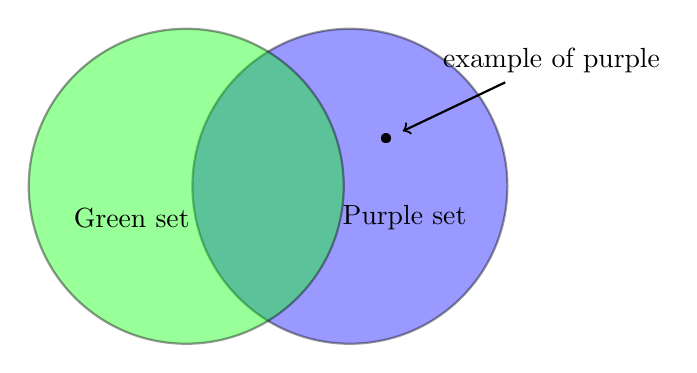
\begin{tikzpicture}[clip=false]
		\fill[blue, draw=black, thick, opacity=.4]  (330:1.2) circle (2);
		\node at ( 330:2)   {Purple set};
		\fill[green, draw=black, thick, opacity=.4] (210:1.2) circle (2);
		\node at ( 210:2)   {Green set};
		
		\uncover<2->{
			\node (C) at (1.5,0) {\textbullet};
			\node (D) at (3.6,1) {example of purple};
			\draw[thick,->] (D) -- (C);
		}
		
		\end{tikzpicture}
	}
	\end{center}
\end{frame}

\begin{frame}{Venn diagram}
	Here's a diagram with the Tikz package: \vspace{.5cm}
	\begin{center}
		\resizebox{4in}{!}{
			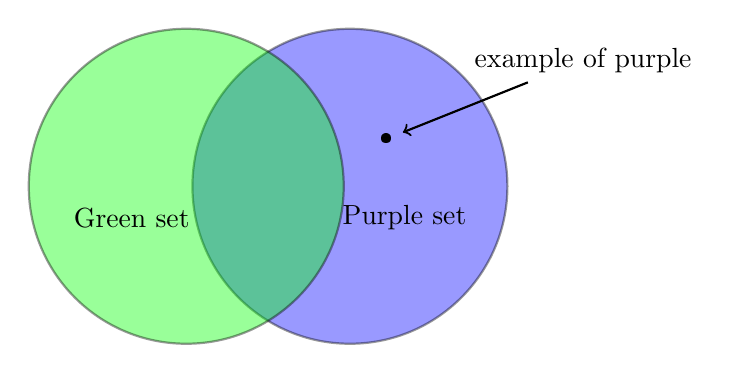
\begin{tikzpicture}[clip=false]
			\fill[blue, draw=black, thick, opacity=.4]  (330:1.2) circle (2);
			\node at ( 330:2)   {Purple set};
			\fill[green, draw=black, thick, opacity=.4] (210:1.2) circle (2);
			\node at ( 210:2)   {Green set};
			
			\uncover<1->{
				\node (C) at (1.5,0) {\textbullet};
				\node (D) at (4,1) {example of purple};
				\draw[thick,->] (D) -- (C);
			}
			
			\end{tikzpicture}
		}
	\end{center}
\end{frame}

\begin{frame}{You can even plot functions}
\begin{figure}[h!]
		\begin{tikzpicture}
		\begin{axis}[
		axis x line=bottom,
		axis y line=left,
		xmin=0, xmax=10, 
		ymin=0, ymax=5,
		xlabel={$y$},
		ylabel={$\phi(y)$}
		]
		\addplot [fill=gray!80, draw=none, domain=0:10, samples=50] {3*gauss(5,1)} \closedcycle;		
		\end{axis}		
		\end{tikzpicture}
	\end{figure}
\end{frame}


\begin{frame}{I like to use TeXstudio}
\begin{center}
 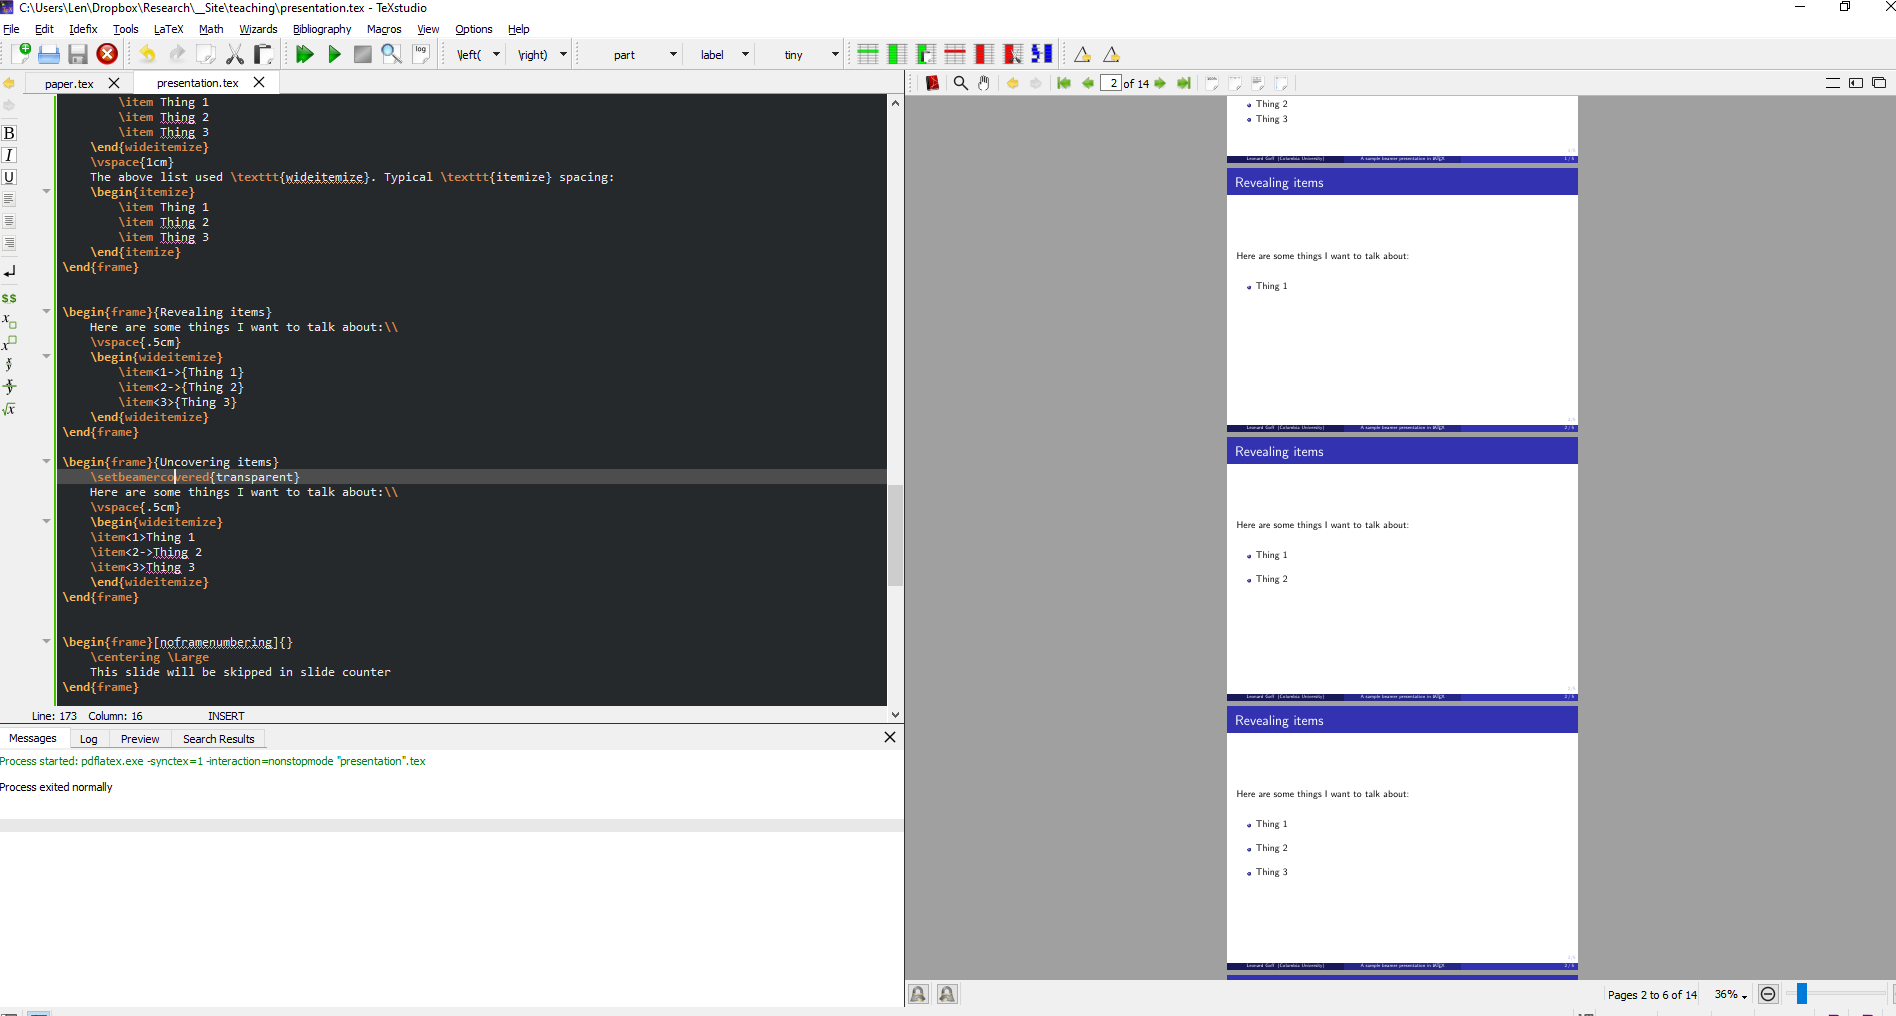
\includegraphics[width=4in]{texstudio}
\end{center}
\end{frame}


\begin{frame}[label=primary]{A typical slide}
	I check from the histogram of X that property P holds approximately. \hyperlink{supplemental}{\beamerbutton{Details}}
\end{frame}

\begin{frame}{Some regression results}
	% Note: including  \usepackage{dcolumn} in preamble was necessary to avoid an error with this Tex file output by stargazer
	\begin{minipage}[t]{\textwidth}
		\tiny
		
% Table created by stargazer v.5.2.2 by Marek Hlavac, Harvard University. E-mail: hlavac at fas.harvard.edu
% Date and time: Wed, Oct 30, 2019 - 11:15:58 AM
% Requires LaTeX packages: dcolumn 
\begin{tabular}{@{\extracolsep{5pt}}lD{.}{.}{-3} D{.}{.}{-3} D{.}{.}{-3} } 
\\[-1.8ex]\hline 
\hline \\[-1.8ex] 
 & \multicolumn{3}{c}{\textit{Dependent variable:}} \\ 
\cline{2-4} 
\\[-1.8ex] & \multicolumn{3}{c}{wage} \\ 
 & \multicolumn{1}{c}{not robust} & \multicolumn{1}{c}{robust} & \multicolumn{1}{c}{robust} \\ 
\\[-1.8ex] & \multicolumn{1}{c}{(1)} & \multicolumn{1}{c}{(2)} & \multicolumn{1}{c}{(3)}\\ 
\hline \\[-1.8ex] 
 employment & 0.023^{***} & 0.023^{***} & 0.023^{***} \\ 
  & (0.001) & (0.005) & (0.005) \\ 
  & & & \\ 
 unemp &  &  & -399.665^{***} \\ 
  &  &  & (50.053) \\ 
  & & & \\ 
 Constant & 23,452.380^{***} & 23,452.380^{***} & 25,647.870^{***} \\ 
  & (104.080) & (171.421) & (359.606) \\ 
  & & & \\ 
\hline \\[-1.8ex] 
Observations & \multicolumn{1}{c}{3,216} & \multicolumn{1}{c}{3,216} & \multicolumn{1}{c}{3,207} \\ 
R$^{2}$ & \multicolumn{1}{c}{0.206} & \multicolumn{1}{c}{0.206} & \multicolumn{1}{c}{0.227} \\ 
Adjusted R$^{2}$ & \multicolumn{1}{c}{0.205} & \multicolumn{1}{c}{0.205} & \multicolumn{1}{c}{0.226} \\ 
Residual Std. Error & \multicolumn{1}{c}{5,700.850 (df = 3214)} & \multicolumn{1}{c}{5,700.850 (df = 3214)} & \multicolumn{1}{c}{5,630.677 (df = 3204)} \\ 
F Statistic & \multicolumn{1}{c}{831.685$^{***}$ (df = 1; 3214)} & \multicolumn{1}{c}{831.685$^{***}$ (df = 1; 3214)} & \multicolumn{1}{c}{469.627$^{***}$ (df = 2; 3204)} \\ 
\hline 
\hline \\[-1.8ex] 
\textit{Note:}  & \multicolumn{3}{r}{$^{*}$p$<$0.1; $^{**}$p$<$0.05; $^{***}$p$<$0.01} \\ 
\end{tabular} 

	\end{minipage}
\end{frame}

\appendix
\backupbegin

\begin{frame}{}
\centering \Large
Extra Slides
\end{frame}


\begin{frame}[label=supplemental]{An extra slide}

\hyperlink{primary}{\beamerbutton{Back}}
\end{frame}


\backupend

\end{document}
			